% Use the custom class defined in GDTReportClass.cls
\documentclass{GDTReportClass}

% Set document metadata using custom commands from the class file
\title{CMLS - Computer Music: Language and System}  % Main title of the document
\subtitle{Course notes}  % Subtitle

\author{Giacomo De Toni}  % Authors
\ID{273703}  % Student ID numbers
\advisor{}  % Advisor's name

% Embed metadata for the PDF file
\begin{filecontents*}{\jobname.xmpdata}
    \Title{CMLS - Computer Music: Language and System}
    \Author{Giacomo De Toni}
    \Language{en-EN}
    \Keywords{Computer-Music \sep Languages \sep Systems \sep PoliMI \sep course_notes \sep LaTeX}
\end{filecontents*}

\begin{document}

    % Generate the front matter (title page, abstract, table of contents, etc.)
    \input{01_FrontMatter/01_titlePage}     % Title page
    \settingfrontmatter  % Configure front matter settings
    \input{01_FrontMatter/03_summaries}     % Summaries

    % Configure main content settings (resets page numbering, chapter counters, etc.)
    \settingmaincontent  

    % Include the main chapters from separate files
    %! TEX root = main.tex  % Specifies the main document file for multi-file projects

\chapter{Course Introduction}

The course Computer Music: Languages and Systems (Course number: 054283) is designed to provide students with a comprehensive understanding of music programming and digital audio systems. It offers both theoretical lectures and practical laboratory sessions, ensuring a hands-on approach to learning.

\section{Course Organization}

The course is divided into three main parts:

\begin{enumerate}
    \item SuperCollider as a music programming language (8 hours lecture, 6 hours lab, 2 hours Q/A and exam preparation).
    
    \begin{itemize}
        \item Architecture of SuperCollider
        \item Coding in SuperCollider
    \end{itemize}
    
    \item Computer Music Systems and plugin architecture (6 hours lecture, 6 hours lab, 2 hours Q/A and exam preparation).
    
    \begin{itemize}
        \item Digital Audio Workstations (DAWs)
        \item Architecture and development of plugins using the JUCE platform
    \end{itemize}

    \item Interaction Design (8 hours lecture, 8 hours lab, 4 hours Q/A and exam preparation).
    
    \begin{itemize}
        \item Machine-to-machine (M2M) and human-to-machine (H2M) interaction
        \item M2M: MIDI and OSC protocols
        \item H2M: Arduino and Bela platforms
    \end{itemize}
\end{enumerate}

A detailed schedule is available on WeBeep.

\section{Textbooks and Materials}

Since computer music is a broad research field, no single textbook covers all topics of the course. Instead, students will rely on:

\begin{itemize}
    \item Course slides, which provide comprehensive coverage.
    \item References at the end of each slide set, some of which are available online.
\end{itemize}

\section{Laboratories}

Laboratory sessions will be held in lecture rooms. Students must install the necessary software on their own laptops, including:

\begin{itemize}
    \item \href{http://supercollider.github.io/download}{SuperCollider}
    \item \href{https://juce.com}{JUCE}
    \item An IDE of choice (Xcode, Visual Studio, etc.)
    \item Arduino, Processing, and other required software
\end{itemize}

\section{Exam and Homework}

The assessment consists of:

\begin{itemize}
    \item A homework assignment (max 14 points), where students develop:
    \begin{itemize}
        \item A synth/effect in SuperCollider
        \item A plugin in JUCE
        \item Interaction via MIDI/OSC and hardware interfaces (Arduino, Bela, etc.)
    \end{itemize}
    \item A written exam (max 18 points), which includes:
    \begin{itemize}
        \item Theoretical questions
        \item Practical exercises on SuperCollider, JUCE, and interaction design
    \end{itemize}
\end{itemize}

Homework is done in groups (3–5 students). A GitHub repository will be used for submission. The final presentation will be graded based on implementation quality, presentation skills, and creativity.  % Chapter 1
    %! TEX root = main.tex  % Specifies the main document file for multi-file projects

\chapter{Computer Music}

There are multiple perspectives on defining computer music:

\begin{itemize}
    \item According to Wikipedia, it is \textit{"music generated or composed with the aid of computers."}
    \item The Columbia University Press defines it as \textit{"music composed or performed with the aid of a computer."}
\end{itemize}

A common understanding emerges: computer music involves the use of computers in music creation, composition, and performance.

\section{Different Approaches to Computer Music}

By searching online for "computer music tutorials," we find two major approaches:

\begin{itemize}
    \item Computer music as music production with computers:
    \begin{itemize}
        \item How to compose music with computers
        \item How to generate sounds with computers
        \item Functional aspects of computer music systems
    \end{itemize}
    \item Computer music as experimental compositions:
    \begin{itemize}
        \item The role of a digital music composer
        \item Exploring new composition tools
    \end{itemize}
\end{itemize}

For further reading, visit:

\begin{itemize}
    \item \href{http://www.computer-music.com/articles/artcl001.htm}{Computer Music Articles}
    \item \href{http://www.computermusic.co.uk/page/computermusic?entry=cm_tutorial_pdfs}{Computer Music Tutorials}
    \item \href{http://musicmall.com/cmp/tutindex.htm}{Music Mall - Tutorials}
    \item \href{http://x2.i-dat.org/~csem/UNESCO/}{UNESCO Computer Music Resources}
    \item \href{http://www.nusystems.co.uk/music/20360/Composing+Music+with+Computers.htm}{Composing Music with Computers}
\end{itemize}

\section{Why "Computer AND Music"?}

The term computer music combines two distinct concepts: 

\begin{itemize}
    \item Computer: a machine designed to manipulate data according to a set of instructions.
    \item Music: an organized form of sound that conveys emotions, thoughts, and impressions.
\end{itemize}

Understanding computer music requires recognizing the synergy between these two disciplines.

\begin{figure}[!htb]
    \centering
    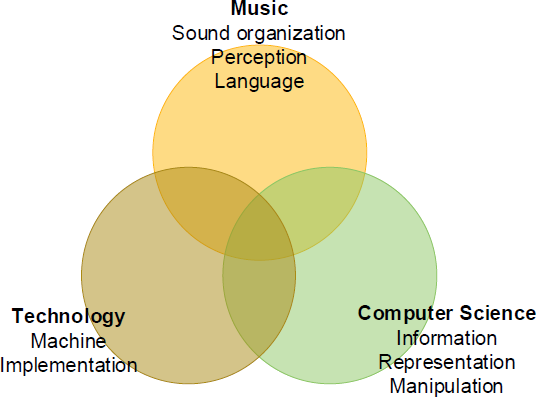
\includegraphics[width=0.6\linewidth]{00_Images/Res/02_chapter/01.png}
    \caption{Computer and music}
    \label{fig:computerandmusic}
\end{figure}

\subsection{Music}

Music can be defined in different ways:

\begin{itemize}
    \item Organized sound: Edgard Varèse defined music as "organized sound," where the organizer (musician, singer, composer, listener) plays a fundamental role.
    \item A category of perception: Music is deeply connected to human cognition.
    \item A language: Music is a form of communication that expresses moods, emotions, and thoughts.
\end{itemize}

\subsection{Computer Science}

A computer is a machine that manipulates data according to a list of instructions. The field of computing, as defined by the Association for Computing Machinery (ACM), is:

\begin{quote}
    "The systematic study of algorithmic processes that describe and transform information, including their theory, analysis, design, efficiency, implementation, and application."
\end{quote}

Computing involves:

\begin{itemize}
    \item Information representation
    \item Information manipulation
    \item Algorithmic processing
\end{itemize}

\subsection{Bringing Everything Together}

Computer music is the intersection of three key domains:

\begin{itemize}
    \item Music: Sound organization, perception, language.
    \item Computer Science: Information representation and manipulation.
    \item Technology: Machines and their implementation in creative processes.
\end{itemize}

This interdisciplinary approach forms the foundation of the course, preparing students to engage with music through computational and technological means.

\section{History of Computer Music}

\subsection{Early Mechanical and Electronic Instruments}

Before digital computers, various automatic instruments paved the way:

\begin{itemize}
    \item Ancient: Greek Aeolian Harp (2nd century BC), mechanical organs (1500s).
    \item 19th-20th Century: Electromechanical Piano (1867), Theremin (1920).
    \item 1950s: RCA Synthesizer (1959) and voltage-controlled synthesizers (1960s).
\end{itemize}

\subsection{The First Computer-Generated Music}

CSIRAC (1949) was the first computer to play music, programmed by Geoff Hill in Australia.

ILLIAC Suite (1957) by Lejaren Hiller and Leonard Isaacson was the first computer-composed piece.

\subsection{Major Developments in Computer Music}

\begin{itemize}
    \item 1957: Max Mathews developed Music I, the first digital sound synthesis program.
    \item 1976: IRCAM was founded in Paris, becoming a leading center for computer music research.
    \item 1983: The MIDI protocol standardized communication between digital instruments.
    \item 1986: Miller Puckette developed Max, the first graphical programming environment for music.
    \item 1989-1991: The rise of Digital Audio Workstations (Sound Tools, Cubase, Pro Tools) revolutionized music production.
\end{itemize}
  % Chapter 2
    %! TEX root = main.tex  % Specifies the main document file for multi-file projects

\chapter{SuperCollider ecosystem}

SuperCollider is an engine for sound synthesis and algorithmic music composition. It provides a real-time sound-based object-oriented programming language, making it suitable for various applications such as music and acoustic research, algorithmic composition, dynamic programming, and live audio coding.

\begin{figure}[!htb]
    \centering
    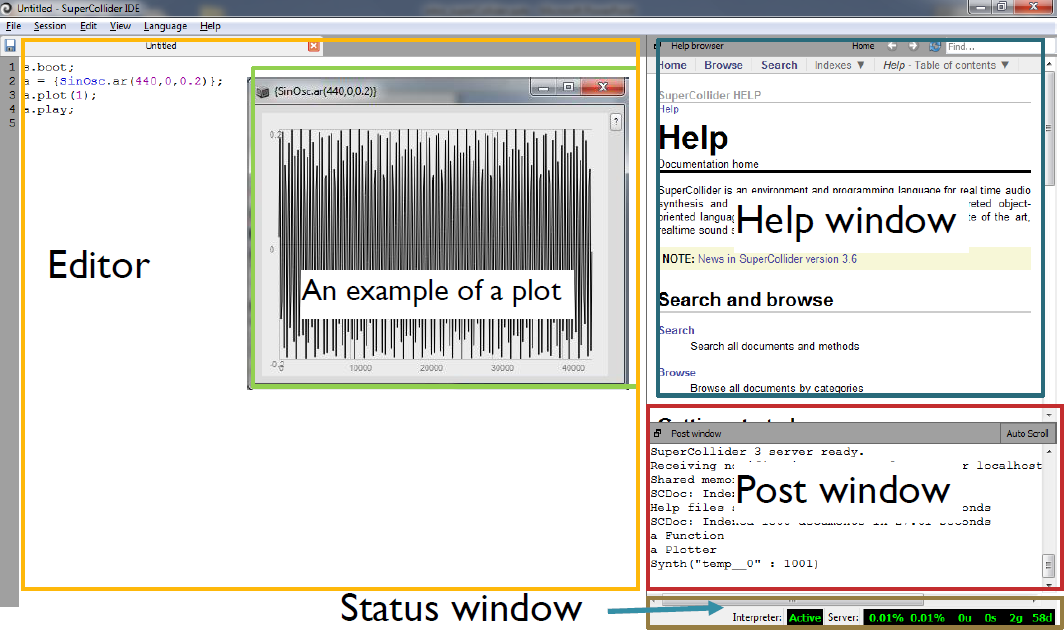
\includegraphics[width=0.8\linewidth]{00_Images/Res/03_chapter/01.png}
    \caption{Appearance of SuperCollider}
    \label{fig:appearance}
\end{figure}

\section{Architecture of SuperCollider}

SuperCollider consists of two main components: a server (scsynth) and a client (sclang), which communicate through OSC (OpenSound Control) messages using TCP/UDP protocols. Additionally, it includes an Integrated Development Environment (IDE).

\subsection{Client and Server}

\begin{itemize}
    \item The server (scsynth) is responsible for sound generation.
    \item The client (sclang) interprets the language and provides a more user-friendly interface.
    \item Typically, both components run on the same machine and communicate via localhost (127.0.0.1), but they can also operate on separate machines.
\end{itemize}

\begin{figure}[!htb]
    \centering
    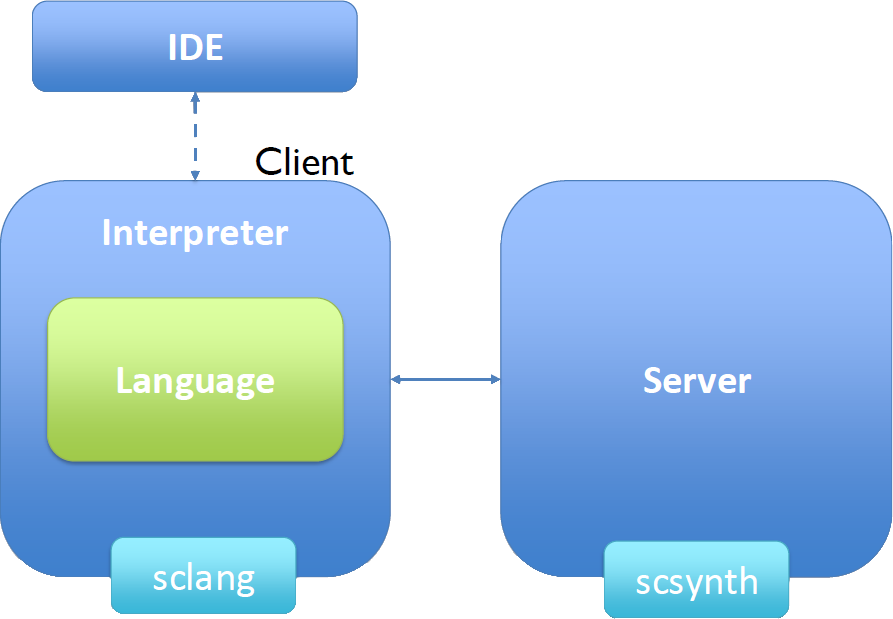
\includegraphics[width=0.5\linewidth]{00_Images/Res/03_chapter/02.png}
    \caption{Interaction between the components}
    \label{fig:interactionserverclient}
\end{figure}

\subsection{Client}

The SC Language (sclang) combines elements of Smalltalk (object-oriented programming) and functional programming. Its syntax follows a C-style structure.

\subsection{Server}

The server is a highly optimized command-line executable, scsynth. Although primarily controlled from within SuperCollider, it can also be used independently. Key features:

\begin{itemize}
    \item Uses OSC for communication.
    \item Supports multiple input and output channels, including large multichannel setups.
    \item Implements a bus system.
    \item Includes buffers for reading and writing.
    \item Operates at three different computation rates: audio rate, control rate, and demand rate.
\end{itemize}

\subsection{SuperCollider IDE}

The Integrated Development Environment (available from version 3.6) includes several components:

\begin{itemize}
    \item Help window.
    \item Post window.
    \item Status window.
    \item Code editor.
    \item Plot visualization tools.
\end{itemize}

SuperCollider is an interpreted language rather than a compiled one. It allows running single lines of code by positioning the cursor on the line and pressing Cmd + Return (MacOS) or Shift + Return (Windows). To stop all server processes, press Cmd + . (MacOS) or Shift + . (Windows).

\subsection{Component Interaction}

SuperCollider's main components interact as follows:

\begin{itemize}
    \item IDE: Provides a graphical user interface.
    \item Interpreter: Executes the SuperCollider language (sclang).
    \item Server (scsynth): Handles audio processing.
    \item Client: Interfaces between the language and the server.
\end{itemize}

\section{The Architecture of the Server}

\subsection{Overview}

The SuperCollider server, scsynth, is an audio synthesis engine that features:

\begin{itemize}
    \item Programmable capabilities.
    \item Real-time audio processing.
\end{itemize}

In scsynth, sound synthesis is achieved through the cooperation of multiple synth objects. The corresponding object in sclang is called Synth. To generate an audio signal, a synth requires processing and synthesis algorithms, which are implemented using UGens (Unit Generators). A UGen is a software module that processes and synthesizes an audio signal. For example, SinOsc is a UGen that generates a sine wave. UGens are the most fundamental components in SuperCollider, analogous to atoms in chemistry. In sclang, items are denoted with uppercase names, whereas in scsynth, their corresponding entities use lowercase names.

\subsection{Synth Creation and UGen Graphs}

To create a new synthesizer, the server requires information about:

\begin{itemize}
    \item The UGens that compose the Synth.
    \item The relationships between these UGens.
\end{itemize}

This information is provided by the client as a UGen graph. In SuperCollider, this is implemented through code, whereas other environments, such as Max/MSP, use graphical representations. A key requirement in SuperCollider is the ability to reuse Synth definitions multiple times. 

\begin{itemize}
    \item The effort to define UGens and their relationships should be done once.
    \item The same Synth structure can be reused with modifications to parameters.
\end{itemize}

For this purpose, SuperCollider provides the SynthDef object, which allows parameter tuning for individual Synth instances.

\begin{figure}[!htb]
    \centering
    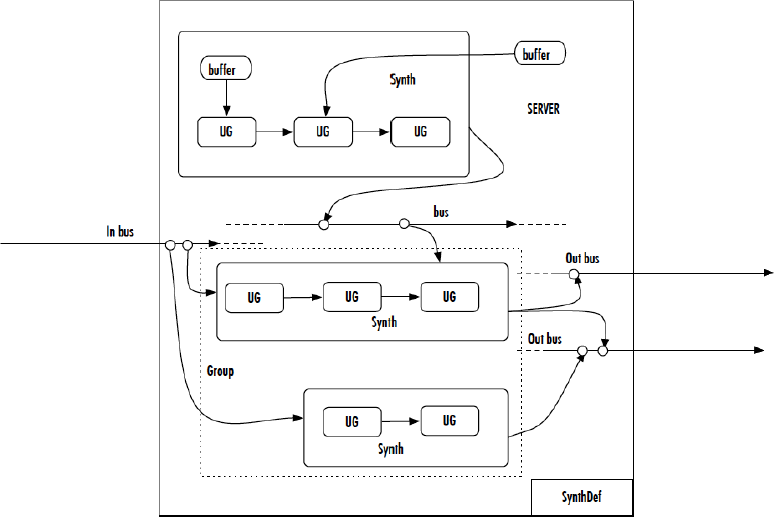
\includegraphics[width=0.8\linewidth]{00_Images/Res/03_chapter/03.png}
    \caption{Example of UGen graph}
    \label{fig:ugengraph}
\end{figure}

\subsection{Synth Communication via Busses}

Multiple Synths interact using busses. Example scenario:

\begin{itemize}
    \item Synth A receives a signal from a microphone and processes it.
    \item The processed signal from Synth A is sent to Bus O.
    \item Synth B retrieves the signal from Bus O, processes it, and sends the output to a special output bus connected to the soundcard.
    \item Synth C processes an audio file and sends the output directly to the output bus.
\end{itemize}

To ensure proper execution, the following conditions must be met:

\begin{itemize}
    \item Synth A must process its signal before Synth B.
    \item Synth A and Synth B must share a private bus that no other Synth can send audio to.
    \item Special busses must be dedicated to input and output signals.
    \item Buffers must be available for reading and writing files.
\end{itemize}

\subsection{Execution Control and Resource Management}

SuperCollider provides mechanisms for:

\begin{itemize}
    \item Controlling the execution order of Synths.
    \item Managing busses for inter-synth communication.
    \item Handling buffers for file operations.
    \item Grouping Synths to manage signal processing workflows.
\end{itemize}

\section{The SuperCollider Language}

\subsection{Object-Oriented Programming in SuperCollider}

SuperCollider follows an object-oriented programming paradigm where:

\begin{itemize}
    \item Objects have properties that can be manipulated.
    \item Objects exchange messages.
    \item Methods define object functionalities for receiving messages and performing operations.
    \item Objects are instances of classes. For example, \texttt{sine1} and \texttt{sine2} can be instances of the \texttt{SinOsc} class, each with different properties despite belonging to the same class.
\end{itemize}

Classes in SuperCollider are organized hierarchically. For example:

\begin{itemize}
    \item \texttt{SinOsc} inherits properties from \texttt{UGen}, a generic signal generator.
    \item Child classes can override parent methods and introduce new properties. For instance, \texttt{SinOsc} adds the \texttt{frequency} property, which \texttt{UGen} does not have.
    \item Some parent class methods can be virtual, meaning they require implementation in child classes.
\end{itemize}

\subsection{Class Notation and Constructors}

\begin{itemize}
    \item Class names start with an uppercase letter. For example, \texttt{Array} is a predefined class for data collections.
    \item Instances of a class are created using constructors. Example:
    
    \begin{supercollider*}
    z = Array.new;
    \end{supercollider*}
    
    \item Some classes have multiple constructors. Example:
    
    \begin{supercollider*}
    z = Array.newClear(indexedSize:12); // Creates an array of 12 elements.
    \end{supercollider*}
    
    \item To check the class of an instance:
    
    \begin{supercollider*}
    z.class;
    \end{supercollider*}
    
    \item To print a class inheritance tree:
    
    \begin{supercollider*}
    Collection.dumpClassSubTree;
    \end{supercollider*}
\end{itemize}

\subsection{Methods and Messages}

Methods in SuperCollider are invoked using the dot notation. Example:

\begin{supercollider*}
z.at(index); // Returns the element at position index.
\end{supercollider*}

To list all methods of a class:

\begin{supercollider*}
ClassName.dumpInterface;
ClassName.dumpFullInterface;
ClassName.dumpMethodList;
\end{supercollider*}

\subsection{Using Methods and Message Chaining}

Example of reversing an array and applying transformations:

\begin{supercollider*}
z = [1,2,3,4];
z.reverse;
z = z.reverse;
z.reverse.mirror.mirror;
\end{supercollider*}

Output:

\begin{supercollider*}
[ 4, 3, 2, 1 ]
[ 1, 2, 3, 4 ]
[ 1, 2, 3, 4, 3, 2, 1, 2, 3, 4, 3, 2, 1 ]
\end{supercollider*}

\subsection{Debugging with postln}

The \texttt{postln} method prints intermediate results:

\begin{supercollider*}
z = [4,3,2,1];
z.postln.reverse.postln.mirror.postln.mirror.postln;
\end{supercollider*}

\subsection{Code Execution and Delimiters}

To execute multiple instructions at once, use parentheses:

\begin{supercollider*}
(
var freq = 440;
SinOsc(freq);
)
\end{supercollider*}

SuperCollider executes one expression at a time, where expressions are delimited by a semicolon.

\subsection{Comments}

\begin{itemize}
    \item Inline comments use \texttt{//}, ignoring text until the end of the line.
    \item Block comments use \texttt{/* */} and can span multiple lines.
\end{itemize}

\subsection{Strings and Variables}

\begin{itemize}
    \item Strings are enclosed in double quotes:
    
    \begin{supercollider*}
    "hello world";
    \end{supercollider*}
    
    \item Variables must be declared, except single-letter variables (\texttt{a-z}).
    \item Local variables are defined using \texttt{var}:
    
    \begin{supercollider*}
    var array = [1,2,3];
    \end{supercollider*}
    
    \item Environment variables use \texttt{\~} instead of \texttt{var}:
    
    \begin{supercollider*}
    ~array = [1,2,3];
    \end{supercollider*}
\end{itemize}

\subsection{Symbols}

Symbols uniquely represent objects:

\begin{supercollider*}
a = \symbol;
b = 'I am a symbol';
a.class;
\end{supercollider*}

\subsection{Functions}

Functions are enclosed in curly brackets:

\begin{supercollider*}
f = { 5 };
f.value; // Returns 5
\end{supercollider*}

Arguments are defined using \texttt{arg}:

\begin{supercollider*}
g = { arg input; input * 2 };
g.value(2); // Returns 4
\end{supercollider*}

Functions can return complex expressions:

\begin{supercollider*}
h = { arg a, b; (a.pow(2) + b.pow(2)).sqrt };
h.value(4,3); // Returns 5
\end{supercollider*}

\subsection{Flow Control}

Example of an if statement:

\begin{supercollider*}
var a = 1, z;
z = if (a < 5, { 100 }, { 200 });
z.postln;
\end{supercollider*}

Example of a while loop:

\begin{supercollider*}
i = 0;
while ( { i < 5 }, { i = i + 1; [i, "boing"].postln });
\end{supercollider*}

Example of a for loop:

\begin{supercollider*}
for (3, 7, { arg i; i.postln });
forBy (0, 8, 2, { arg i; i.postln });
\end{supercollider*}

\subsection{Interacting with the Server}

Basic server commands:

\begin{supercollider*}
s.boot; // Start the server
s.quit; // Stop the server
s.reboot; // Restart the server
\end{supercollider*}

Visualizing signals:

\begin{supercollider*}
s.scope; // Time-domain visualization
s.freqscope; // Frequency-domain visualization
\end{supercollider*}

\subsection{Creating and Controlling Sound}

A simple sinusoidal signal:

\begin{supercollider*}
{ SinOsc.ar(440, 0, 0.2) }.play;
\end{supercollider*}

Modifying amplitude dynamically:

\begin{supercollider*}
(
{ var ampOsc;
  ampOsc = SinOsc.kr(0.5, 1.5pi, 0.5, 0.5);
  SinOsc.ar(440, 0, ampOsc);
}.play;
)
\end{supercollider*}

\subsection{Stereo Output and Panning}

Basic stereo signal:

\begin{supercollider*}
{ [SinOsc.ar(440, 0, 0.2), SinOsc.ar(442, 0, 0.2)] }.play;
\end{supercollider*}

Using multichannel expansion:

\begin{supercollider*}
{ SinOsc.ar([440, 442], 0, 0.2) }.play;
\end{supercollider*}

Randomized frequency selection:

\begin{supercollider*}
(
{ var freq;
  freq = [[660, 880], [440, 660], 1320, 880].choose;
  SinOsc.ar(freq, 0, 0.2);
}.play;
)
\end{supercollider*}

Using Pan2 for panning:

\begin{supercollider*}
{ Pan2.ar(PinkNoise.ar(0.2), SinOsc.kr(0.5)) }.play;
\end{supercollider*}
  % Chapter 3
    %! TEX root = main.tex  % Specifies the main document file for multi-file projects

\chapter{SuperCollider as a Computer Music Language}

\section{Synth and SynthDef}

\subsection{Creating a SynthDef}

A SynthDef defines a new type of synthesizer in SuperCollider. The following example creates a simple SynthDef that outputs a sine wave:

\begin{supercollider*}
SynthDef.new("bee",
{ Out.ar(0, SinOsc.ar(440)) }
).add;
\end{supercollider*}

Explanation:

\begin{itemize}
    \item \texttt{SynthDef.new} creates a new SynthDef.
    \item \texttt{"bee"} is the name of this SynthDef.
    \item \texttt{Out.ar(0, SinOsc.ar(440))} sends the output of a sinusoidal oscillator to bus 0.
    \item \texttt{SinOsc.ar(440)} generates a sine wave at 440 Hz.
    \item \texttt{add} loads the SynthDef onto the server but does not save it to disk.
\end{itemize}

\begin{figure}[!htb]
    \centering
    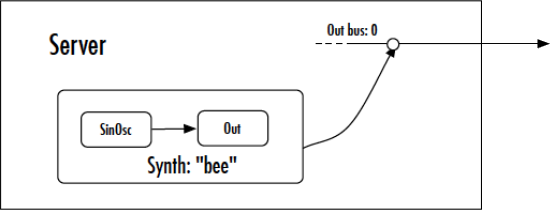
\includegraphics[width=0.7\linewidth]{00_Images/Res/04_chapter/01.png}
    \caption{bee SynthDef}
    \label{fig:beeSynthDef}
\end{figure}

\subsection{Signal Flow and UGen Graph}

Each SynthDef is represented as a UGen graph, which describes the relationships between unit generators and their parameters.

\subsection{SynthDef Arguments}

To allow parameter variation between different instances of a Synth, arguments can be added:

\begin{supercollider*}
SynthDef.new(\pulseSine, { arg out = 0, amp = 0.25, kfreq = 5;
    Out.ar(
        bus: out,
        channelsArray: SinOsc.ar(
            freq: kfreq * 50,
            mul: LFPulse.kr(freq: kfreq, width: 0.25)
        ) * amp
    );
}).add;
\end{supercollider*}

\begin{figure}[!htb]
    \centering
    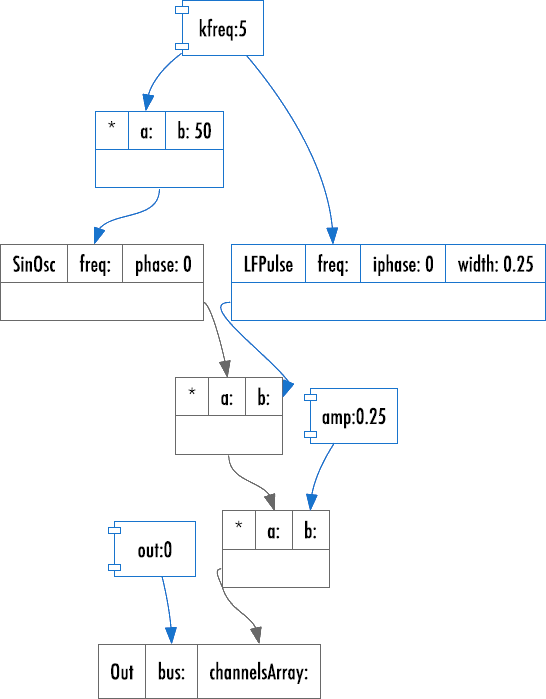
\includegraphics[width=0.6\linewidth]{00_Images/Res/04_chapter/02.png}
    \caption{SynthDef arguments}
    \label{fig:synthdefarguments}
\end{figure}

\subsection{Explanation of Arguments}

\begin{itemize}
    \item \texttt{arg out = 0, amp = 0.25, kfreq = 5;} declares default values for the arguments.
    \item \texttt{Out.ar(bus: out, channelsArray: ...)} assigns the output to the specified bus.
    \item \texttt{LFPulse.kr(freq: kfreq, width: 0.25)} generates a low-frequency pulse wave at control rate.
    \item The resulting Synth produces a sine wave that is periodically switched on and off based on the pulse wave.
\end{itemize}

\subsection{Creating a Synth from a SynthDef}

Once a SynthDef is defined, it can be instantiated as follows:

\begin{supercollider*}
c = Synth.new("pulseSine"); // Create and play the synth
d = Synth.newPaused(\pulseSine); // Create but do not play the synth
d.run(true); // Start the synth
d.run(false); // Pause the synth
d.set(\kfreq, 9); // Modify a parameter
d.free; // Deallocate the synth
\end{supercollider*}

\subsection{Mouse-Based Theremin}

This example maps mouse movement to control pitch and amplitude:

\begin{supercollider*}
SynthDef.new(\theremin, {
    Out.ar(0,
        SinOsc.ar(
            freq: MouseX.kr(200, 5000, 1),
            mul: MouseY.kr(0,1)
        )
    )
}).add;
\end{supercollider*}

Explanation:

\begin{itemize}
    \item \texttt{MouseX.kr(200, 5000, 1)} maps the horizontal mouse position to frequency.
    \item \texttt{MouseY.kr(0,1)} maps the vertical mouse position to amplitude.
\end{itemize}

\begin{figure}[!htb]
    \centering
    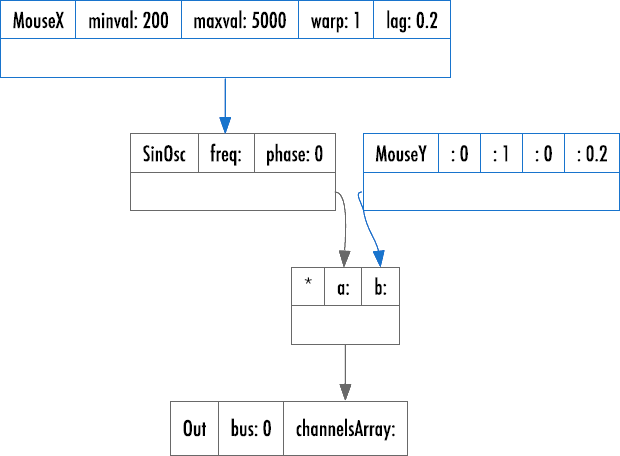
\includegraphics[width=0.55\linewidth]{00_Images/Res/04_chapter/03.png}
    \caption{Mouse-based theremin ugen graph}
    \label{fig:mouse-basedtheremin}
\end{figure}

\subsection{Implicit SynthDef}

SuperCollider allows playing a Synth without explicitly defining a SynthDef:

\begin{supercollider*}
{ SinOsc.ar(440, 0, 0.2) }.play;
\end{supercollider*}

When executed, a temporary SynthDef named \texttt{temp\_\_0} is automatically generated by SuperCollider. This method is useful for quick testing but inefficient for complex Synths.

\section{Controlling the Envelope of a Signal}

\subsection{Defining the Envelope Prototype}

SuperCollider allows controlling the temporal envelope of a signal using the \texttt{Env} class. The following example defines an envelope prototype:

\begin{supercollider*}
e = Env.new(
    levels:[0.0, 1.0, 0.5, 0.5, 0.0],
    times: [0.05, 0.1, 0.5, 0.35]
).plot;
\end{supercollider*}

This defines an ADSR-like envelope:

\begin{itemize}
    \item Attack lasts 0.05s, reaching a peak of 1.
    \item Decay lasts 0.1s, reducing the level to 0.5.
    \item Sustain lasts 0.5s at level 0.5.
    \item Release lasts 0.35s, fading to 0.
\end{itemize}

\begin{figure}[!htb]
    \centering
    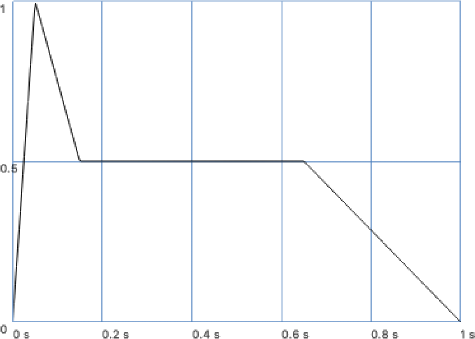
\includegraphics[width=0.7\linewidth]{00_Images/Res/04_chapter/04.png}
    \caption{Defining the envelope prototype}
    \label{fig:envelopeprototype}
\end{figure}

\subsection{Generating the Envelope with EnvGen}

The \texttt{EnvGen} class is used to apply the envelope to a signal at audio or control rate:

\begin{supercollider*}
EnvGen.ar(envelope, gate: 1, levelScale: 1, levelBias: 0, timeScale: 1, doneAction: 0)
EnvGen.kr(envelope, gate: 1, levelScale: 1, levelBias: 0, timeScale: 1, doneAction: 0)
\end{supercollider*}

Arguments:

\begin{itemize}
    \item \texttt{envelope}: An envelope created with \texttt{Env}.
    \item \texttt{gate}: Triggers the envelope each time the signal crosses zero in the positive direction.
    \item \texttt{levelScale}: Scales the amplitude.
    \item \texttt{levelBias}: Adds an offset to the amplitude.
    \item \texttt{timeScale}: Stretches (\textgreater1) or compresses (\textless1) the duration.
    \item \texttt{doneAction}: Defines the behavior at the end. \texttt{doneAction = 2} frees the synth, while \texttt{doneAction = 0} keeps it active.
\end{itemize}

\subsection{Examples of Envelope Application}

Using \texttt{EnvGen} to control amplitude:

\begin{supercollider*}
~env = Env.new(
    levels:[0.0, 1.0, 0.5, 0.5, 0.0],
    times: [0.05, 0.1, 0.5, 0.35]
);

{ SinOsc.ar(440) * EnvGen.kr(~env, 1, 1, 0, 1, 0) }.plot(2);
\end{supercollider*}

Modifying time and level scaling:

\begin{supercollider*}
{ SinOsc.ar(440) * EnvGen.kr(~env, 1, 2, 0, 2, 0) }.plot(2);
\end{supercollider*}

\subsection{Gating the Envelope}

The \texttt{gate} argument can be dynamically controlled. This example restarts the envelope every second using a low-frequency sine wave:

\begin{supercollider*}
~env = Env.new(
    levels:[0.0, 1.0, 0.5, 0.5, 0.0],
    times: [0.05, 0.1, 0.5, 0.35]
);

{ SinOsc.ar(440) * EnvGen.kr(~env, SinOsc.kr(1), 1, 0, 1, 0) }.plot(2);
\end{supercollider*}

\subsection{Predefined Envelope Types}

SuperCollider provides several built-in envelope types:

\begin{itemize}
    \item \texttt{Env.linen(atkT, sustT, relT, level, curve)}: Trapezoidal shape (no decay).
    \item \texttt{Env.triangle(dur, level)}: Triangular shape.
    \item \texttt{Env.sine(dur, level)}: Hanning window shape.
    \item \texttt{Env.perc(atkT, relT, level, curve)}: Typically percussive shape.
\end{itemize}

More envelope types can be found in the SuperCollider reference guide.

\section{Bus Management}

\subsection{Introduction to Busses}

Busses in SuperCollider are named after the analog mixing desk busses and are used to route signals between the audio hardware or different synths. There are two types of busses:

\begin{itemize}
    \item Audio rate busses, which transmit signals at the audio rate.
    \item Control rate busses, which transmit lower-frequency control signals.
\end{itemize}

\subsection{Bus Indexing}

Busses are accessed using numerical indices:

\begin{itemize}
    \item Control rate busses start from index \texttt{0}.
    \item Audio rate busses are indexed more complexly:
    
    \begin{itemize}
        \item The first \texttt{n} channels correspond to physical input and output busses, where:
        
        \begin{supercollider*}
        n = server.options.numOutputBusChannels + server.options.numInputBusChannels
        \end{supercollider*}
        
        \item Indices from \texttt{0} to \texttt{server.options.numOutputBusChannels -1} are hardware output busses.
        \item Indices from \texttt{server.options.numOutputBusChannels} onward are hardware input busses.
        \item The remaining indices are private busses for inter-synth communication.
    \end{itemize}
\end{itemize}

\subsection{Accessing Busses for Input and Output}

To write to an audio rate bus, use \texttt{Out.ar}:

\begin{supercollider*}
Out.ar(out, channelsArray);
\end{supercollider*}

\begin{itemize}
    \item \texttt{out} is the index of the target bus.
    \item \texttt{channelsArray} is the signal to be routed. If multichannel, the channels are mapped to consecutive busses.
\end{itemize}

To read from an audio rate bus, use \texttt{In.ar}:

\begin{supercollider*}
In.ar(bus: 0, numChannels: 1);
\end{supercollider*}

\begin{itemize}
    \item \texttt{bus} is the index of the first bus to read from.
    \item \texttt{numChannels} specifies how many consecutive busses to read.
\end{itemize}

Similar methods exist for control rate busses: \texttt{In.kr} and \texttt{Out.kr}.

\subsection{Example: Mixing Signals on the Same Bus}

When multiple synths write to the same bus, their outputs are mixed:

\begin{supercollider*}
(
SynthDef(\sine_mix, { arg freq = 440, out = 0;
    Out.ar(out, SinOsc.ar(freq, 0, 0.2));
}).send(s);
)

// Both synths write to bus 1, and their outputs are mixed
x = Synth(\sine_mix, ["out", 1, "freq", 660]);
y = Synth(\sine_mix, ["out", 1, "freq", 770]);
\end{supercollider*}

\subsection{Allocating Busses}

Busses can be allocated dynamically using the \texttt{Bus} class:

\begin{supercollider*}
// Allocate a 2-channel control bus
b = Bus.control(s, 2);

// Allocate a private audio bus
c = Bus.audio(s);
\end{supercollider*}

To read and write from these busses, use \texttt{Out.kr}, \texttt{Out.ar}, \texttt{In.kr}, and \texttt{In.ar}.

\subsection{Working with Busses}

\begin{supercollider*}
b = Bus.control(s, 2); // Create a 2-channel control bus
b.index; // Get the bus index
b.numChannels; // Get the number of channels

b.free; // Free the allocated bus
\end{supercollider*}

\subsection{Example: Using Busses to Control Frequency}

\begin{supercollider*}
(
SynthDef("tutorial-Infreq", { arg bus, freqOffset = 0;
    Out.ar(0, SinOsc.ar(In.kr(bus) + freqOffset, 0, 0.5));
}).send(s);

SynthDef("tutorial-Outfreq", { arg freq = 400, bus;
    Out.kr(bus, SinOsc.kr(1, 0, freq/40, freq));
}).send(s);

b = Bus.control(s, 1);
)

// Assign synths to bus
x = Synth.new("tutorial-Outfreq", [\bus, b]);
y = Synth.after(x, "tutorial-Infreq", [\bus, b]);
z = Synth.after(x, "tutorial-Infreq", [\bus, b, \freqOffset, 200]);

// Free resources
x.free; y.free; z.free; b.free;
\end{supercollider*}

\subsection{Execution Order Control with after}

\begin{itemize}
    \item Both \texttt{y} and \texttt{z} read from the same control bus \texttt{b}.
    \item \texttt{z} adds an offset of 200 Hz to the frequency.
    \item The \texttt{after} method ensures \texttt{y} and \texttt{z} are executed after \texttt{x}.
\end{itemize}

\section{Groups and Order of Execution}

\subsection{Groups}

In SuperCollider, synths on the server are classified as nodes. Another type of node is a group, which is a collection of nodes that can include both synths and other groups. Groups are useful for:

\begin{itemize}
    \item Controlling the order of execution of synths.
    \item Grouping nodes together to send messages collectively.
\end{itemize}

SuperCollider provides an abstraction object called \texttt{Group} to manage groups in the client application.

\subsection{Controlling the Order of Execution}

Busses facilitate communication between synths, but proper execution order must be maintained. If one synth writes to a bus and another reads from it, the latter must execute afterward to avoid outdated signals.

SuperCollider provides two arguments in \texttt{Synth.new} to control execution placement:

\begin{itemize}
    \item \texttt{target}: The group or synth that determines the execution order.
    \item \texttt{addAction}: Specifies the position of the new synth relative to the target.
\end{itemize}

If no target is provided, the synth is placed in the default group.

\begin{figure}[!htb]
    \centering
    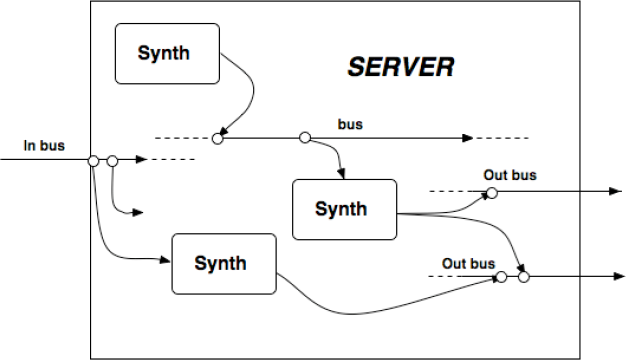
\includegraphics[width=0.7\linewidth]{00_Images/Res/04_chapter/08.png}
    \caption{Controlling the order of execution}
    \label{fig:controllingorder}
\end{figure}

\subsection{Synth Placement Methods}

SuperCollider provides several methods for precise placement of synths:

\begin{supercollider*}
Synth.new(defName, args, target, addAction);
\end{supercollider*}

\begin{itemize}
    \item If \texttt{target} is a synth, \texttt{addToHead} and \texttt{addToTail} place the synth at the beginning or end of the group.
    \item If \texttt{target} is a server, the synth is placed in the server's default group.
    \item If \texttt{target} is \texttt{nil}, it defaults to the main group of the default server.
\end{itemize}

Additional methods:

\begin{supercollider*}
Synth.head(aGroup, defName, args);
\end{supercollider*}

Places the new synth at the head of \texttt{aGroup}.

\begin{supercollider*}
Synth.tail(aGroup, defName, args);
\end{supercollider*}

Places the new synth at the tail of \texttt{aGroup}.

\begin{supercollider*}
Synth.before(aNode, defName, args);
\end{supercollider*}

Adds the new synth just before \texttt{aNode}.

\begin{supercollider*}
Synth.after(aNode, defName, args);
\end{supercollider*}

Adds the new synth just after \texttt{aNode}.

\begin{supercollider*}
Synth.replace(synthToReplace, defName, args);
\end{supercollider*}

Replaces \texttt{synthToReplace} with the new synth and frees the original node.

\subsection{Creating and Managing Groups}

Like synths, groups accept \texttt{target} and \texttt{addAction} arguments for controlled placement.

Example:

\begin{supercollider*}
g = Group.new;        // Create a new group
h = Group.before(g);  // Create a group before g
g.free;              // Free group g
h.free;              // Free group h
\end{supercollider*}

\section{Scheduling Events in SuperCollider}

\subsection{The Problem of Scheduling}

According to Edgar Varèse, music is "organized sound." This implies that musical composition involves two aspects:

\begin{itemize}
    \item Internal organization of sound, such as harmonic content and timbre.
    \item Temporal organization of events, which requires scheduling.
\end{itemize}

SuperCollider provides several methods to manage event scheduling.

\subsection{Scheduling through Pulse Generation}

A sequence of discrete events can be generated using pulse signals.

\begin{supercollider*}
SynthDef.new("pulseEvent", { |seqFreq = 4, sawFreq = 0.125, sinFreq = 0.14| 
    Out.ar(0,
        Pulse.kr(seqFreq, width:0.1, mul:0.5, add:0.5) *
        Formant.ar(
            fundfreq: (LFSaw.kr(sawFreq, mul:6, add:60) + SinOsc.ar(sinFreq, mul:3)).round.midicps
        )
    )
}).add; 

x = Synth.new("pulseEvent", [\seqFreq , 4]);
\end{supercollider*}

\subsection{Pulse and Formant UGens}

\texttt{Pulse.kr(freq, width, mul, add)} generates a band-limited pulse wave:

\begin{itemize}
    \item \texttt{freq}: Pulse frequency in Hz.
    \item \texttt{width}: Pulse width ratio (0.5 produces a square wave).
    \item \texttt{mul}, \texttt{add}: Scaling and offset parameters.
\end{itemize}

\texttt{Formant.ar(fundFreq, formFreq, bwFreq)} generates harmonic signals by filtering harmonics at \texttt{fundFreq}.

\subsection{Scheduling through Envelopes}

Envelopes can be used to create discrete events over time.

\begin{supercollider*}
(
{
    var freq = 422, cycleDur = 2;
    var env = Env([0,1,1,0,0,1,1,0, 0], [0,1,0, 1, 0, 2.5, 0, 1.5]);
    EnvGen.kr(env, 1, gate: Impulse.kr(1/cycleDur), timeScale: 1/5, doneAction: 0) 
    * SinOsc.ar(freq)
}.play
)
\end{supercollider*}

\subsection{Scheduling through Select}

\texttt{Select.kr(which, array)} chooses elements from an array based on an index.

\begin{supercollider*}
SynthDef(\select, {
    var array = Array.fill(64, {|i| (i%4) + (i%7) + (i%11) + 60});
    array = array.add(90).postln.midicps;
    Out.ar(0, Saw.ar(Select.kr(LFSaw.kr(1/6).linlin(-1.0,1.0, 0, array.size).round, array), 0.2));
}).add;

Synth(\select);
\end{supercollider*}

\subsection{Scheduling through the Demand UGen}

\texttt{Demand.kr(trig, reset, [..ugens..])} is triggered when \texttt{trig} becomes true.

\begin{supercollider*}
(
{
    var a, freq, trig;
    a = Dseq([1, 3, 2, 7, 8] + 60, 3);
    trig = Impulse.kr(4);
    freq = Demand.kr(trig, 0, a.midicps);
    Mix.fill(10, { Pulse.ar(freq + 5.rand) }) * 0.1;
}.play;
)
\end{supercollider*}

\subsection{Scheduling through Routine and Clocks}

SuperCollider provides different clocks for event scheduling:

\begin{itemize}
    \item \texttt{SystemClock}: High-priority clock, non-musical timing.
    \item \texttt{TempoClock}: Musical timing, default 60 BPM.
    \item \texttt{AppClock}: Low-priority, used for GUI activities.
\end{itemize}

Example of scheduling with \texttt{SystemClock}:

\begin{supercollider*}
(
"waiting for three seconds".postln;
SystemClock.sched(3.0, { "done".postln });
)
\end{supercollider*}

Example of using \texttt{Routine}:

\begin{supercollider*}
r = Routine.new({
    var time;
    10.do({ |i| 
        "slowing".postln;
        time = (i * 0.1).postln;
        time.wait;
    });
    1.wait;
    "the".postln;
    1.wait;
    "end".postln;
});
SystemClock.play(r);
\end{supercollider*}

\subsection{Using Fork for Scheduling}

Instead of explicitly defining a routine, the \texttt{fork} method schedules a function:

\begin{supercollider*}
(
{
    var amp = 0.125;
    var firstBit = Array.fill(32, {[0,1].choose});
    var secondBit = Array.fill(16, {[0,1].choose});
    var freq;

    firstBit.do{|i|
        freq = [2000, 2500][i];
        { SinOsc.ar(freq, mul: amp) * Line.kr(1,1,0.30, doneAction:2) }.play;
        0.03.wait;
    };

    0.04.wait;

    secondBit.do{|i|
        freq = [2000, 2500][i];
        { SinOsc.ar(freq, mul: amp) * Line.kr(1,1,0.30, doneAction:2) }.play;
        0.03.wait;
    };

    0.52.wait;

    { SinOsc.ar(1000, mul: amp) * LFPulse.ar(1, width:0.1) * Line.kr(1,1,5, doneAction:2) }.play;
    6.wait;
    { SinOsc.ar(1000, mul: amp) * Line.ar(1,1,0.1, doneAction:2) }.play;
}.fork;
)
\end{supercollider*}

\subsection{Scheduling with Patterns}

\texttt{Pseq} describes sequences by repeating a seed sequence.

\begin{supercollider*}
p = Pseq([1,2,3,4], 3).asStream;
13.do{ "next...? -> ".post; p.next.postln };
\end{supercollider*}

Example of using \texttt{Pseq} in a synth:

\begin{supercollider*}
SynthDef(\sinPerc, { |freq = 440, pos = 0, level = 0.125, detune = 0.025|
    var sig = Mix.fill(10, { SinOsc.ar(freq + Rand(0, freq * detune)) });
    sig = FreeVerb.ar(sig * EnvGen.kr(Env.perc));
    DetectSilence.ar(sig, -96.dbamp, doneAction:2);
    Out.ar(0, Pan2.ar(sig, pos, level));
}).add;

(
p = Pseq([0,2,4,3,10,13,12,6,5,7], inf).asStream;
{
    inf.do{
        Synth(\sinPerc, [\freq, (p.next+70).midicps]);
        0.25.wait;
    }
}.fork;
)
\end{supercollider*}

\section{Buffers}

\subsection{Introduction to Buffers}

A buffer is a memory space allocated to store data, typically used for audio storage and manipulation. Buffers in SuperCollider function similarly to busses but are used for sampled data instead of signal routing.

\subsection{Creating and Using Buffers}

A buffer can be allocated using:

\begin{supercollider*}
Buffer.alloc(server, numFrames, numChannels: 1, completionMessage, bufnum)
\end{supercollider*}

Example:

\begin{supercollider*}
(
var buf = Buffer.alloc(s, 2.pow(10));

// Fill buffer with a sine wave
buf.sine1([1]);

// Play the buffer using an oscillator
{Osc.ar(buf, 440)}.play;
)
\end{supercollider*}

\subsection{Buffer Methods}

\texttt{sine1(amps,norm: true,asWavetable: true,clearFirst: true)} fills the\hfill\\buffer with harmonics.

\begin{itemize}
    \item \texttt{amps}: Array of harmonic amplitudes.
    \item \texttt{norm}: Normalizes buffer peak to 1.0 (default: true).
    \item \texttt{asWavetable}: Stores as a wavetable for interpolation (default: true).
    \item \texttt{clearFirst}: Clears the buffer before writing (default: true).
\end{itemize}

For arbitrary phase relationships, use \texttt{sine3}.

\subsection{Oscillator Using Buffers}

The \texttt{Osc} class provides a wavetable lookup oscillator:

\begin{supercollider*}
Osc.ar(bufnum, freq: 440, phase: 0, mul: 1, add: 0)
\end{supercollider*}

\begin{itemize}
    \item \texttt{bufnum}: Buffer variable.
    \item \texttt{freq}: Frequency in Hz.
    \item \texttt{phase}: Phase offset in radians.
    \item \texttt{mul}, \texttt{add}: Scaling and offset parameters.
\end{itemize}

\subsection{Writing and Reading Audio Files}

\paragraph{Writing a File}

The \texttt{Signal} class provides special methods for filling buffers.

\begin{supercollider*}
(
var sig;
var soundFile;

sig = Signal.sineFill(2.pow(16), [1]); // Generate sine wave with 65536 samples
sig = sig.asWavetable; // Convert to wavetable format

soundFile = SoundFile.new;
soundFile.headerFormat_(
    "AIFF").sampleFormat_("int16").numChannels_(1);
soundFile.openWrite("/signalTest.aiff");
soundFile.writeData(sig);
soundFile.close;
)
\end{supercollider*}

\paragraph{Reading a File into a Buffer}

\begin{supercollider*}
(
// Define a synth to read the file
SynthDef("tableOsc", { arg buf, freq = 440, amp = 0.4; 
    Out.ar(0, Osc.ar(buf, freq, mul: amp));
}).add;
)

(
// Allocate buffer and load the file
var freq = 440;
var buf, aSynth;

buf = Buffer.read(s, "/signalTest.aiff");

// Play the buffer
aSynth = Synth.new("tableOsc", ["buf", buf]);
)
\end{supercollider*}

\section{Signal Visualization and GUIs}

\subsection{Scope and Plot}

SuperCollider provides two main methods to visualize signals: \texttt{plot} and \texttt{scope}.

\paragraph{Using plot}

The \texttt{plot} method generates a static graph of a signal:

\begin{supercollider*}
{ PinkNoise.ar(0.2) + SinOsc.ar(440, 0, 0.2) + Saw.ar(660, 0.2) }.plot;
\end{supercollider*}

By default, the plot covers 0.01 seconds, but this can be modified:

\begin{supercollider*}
{ PinkNoise.ar(0.2) + SinOsc.ar(440, 0, 0.2) + Saw.ar(660, 0.2) }.plot(1);
\end{supercollider*}

\paragraph{Using scope}

The \texttt{scope} method provides a real-time oscilloscope visualization:

\begin{supercollider*}
{ PinkNoise.ar(0.2) + SinOsc.ar(440, 0, 0.2) + Saw.ar(660, 0.2) }.scope;
\end{supercollider*}

For multichannel signals:

\begin{supercollider*}
{ [SinOsc.ar(440, 0, 0.2), SinOsc.ar(442, 0, 0.2)] }.scope;
\end{supercollider*}

To adjust zoom:

\begin{supercollider*}
{ [SinOsc.ar(440, 0, 0.2), SinOsc.ar(442, 0, 0.2)] }.scope(zoom: 10);
\end{supercollider*}

\paragraph{Using freqscope}

The \texttt{freqscope} method visualizes the spectrum of the signal:

\begin{supercollider*}
(
{ SinOsc.ar(440) }.play;
s.freqscope;
)
\end{supercollider*}

\subsection{GUI Creation}

SuperCollider allows creating custom graphical interfaces.

\begin{supercollider*}
s.boot;

(
// Define an audio SynthDef
SynthDef.new("square", { arg out = 0, freq = 400, amp = 0.75, width = 0.5;
    Out.ar(out, Pulse.ar(freq, width: width, mul: amp));
}).add;
)

(
// Create GUI elements
var aSynth, window, knob1, knob2, button;

aSynth = Synth.new(\square); 

window = Window.new("Knob", Rect(300, 300, 240, 100));
window.front;

knob1 = Knob.new(window, Rect(30, 30, 50, 50)).valueAction_(0.25);
knob2 = Knob.new(window, Rect(90, 30, 50, 50)).valueAction_(0.3);

button = Button.new(window, Rect(150, 30, 50, 50));
button.states = [["stop", Color.black], ["start", Color.red]];

knob1.action_({arg me; aSynth.set(\amp, me.value) });
knob2.action_({arg me; aSynth.set(\freq, me.value.linlin(0,1, 200, 2000)) });

button.action = ({ arg me;
    var val = me.value.postln;
    if (val == 1) { aSynth.run(false) } { aSynth.run }
});

window.onClose_({ aSynth.free });
)
\end{supercollider*}

\subsection{Sliders in GUIs}

The \texttt{Slider} class provides an alternative control method:

\begin{supercollider*}
Slider.new(parent, bounds);
\end{supercollider*}

\begin{itemize}
    \item \texttt{value} sets the slider position.
    \item \texttt{valueAction} triggers a function on change.
\end{itemize}

\subsection{Advanced Signal Visualization}

\texttt{Stethoscope}, \texttt{FreqScope}, and \texttt{FreqScopeView} provide additional visualization tools.

\begin{supercollider*}
(
var window;
window = Window.new("scope", Rect(300, 300, 540, 300));
window.front;

{ SinOsc.ar(440) }.play;
Stethoscope.new(server: s, numChannels: 2, view: window);
)
\end{supercollider*}

To display a frequency spectrum:

\begin{supercollider*}
(
w = Window("My Analyzer", Rect(0, 0, 511, 300));
f = FreqScopeView(w, w.view.bounds);
f.active_(true);
w.onClose_({ f.kill });
w.front;

{ SinOsc.ar([500, 1000], 0, 0.25) }.play(s);
)
\end{supercollider*}
  % Chapter 4
    %! TEX root = main.tex  % Specifies the main document file for multi-file projects

\chapter{Introduction to Computer Music Systems and Plugins}

\section{Learning Objectives}

This section covers fundamental concepts related to Computer Music Systems, including:

\begin{itemize}
    \item Understanding what a Computer Music Performance System (CMPS) is
    \item Learning the architecture of a CMPS
    \item Exploring the role of sequencers in the composition lifecycle
    \item Analyzing how signal processing systems operate within a sequencer
    \item Understanding how plugins function in a Digital Audio Workstation (DAW), including:
    \begin{itemize}
        \item GUI management
        \item Plugin API interaction
    \end{itemize}
\end{itemize}

\section{Applications of Computer Music Systems}

Computer music has evolved significantly due to progress in computer science and electronics. The main applications of computer music systems include:

\begin{itemize}
    \item Sound generation
    \item Automatic music composition
    \item Audio editing
    \item MIDI transmission, recording, and playback
    \item Sound processing
    \item Live sound processing
\end{itemize}

\section{Computer Music Performance Systems}

\begin{figure}[!htb]
    \centering
    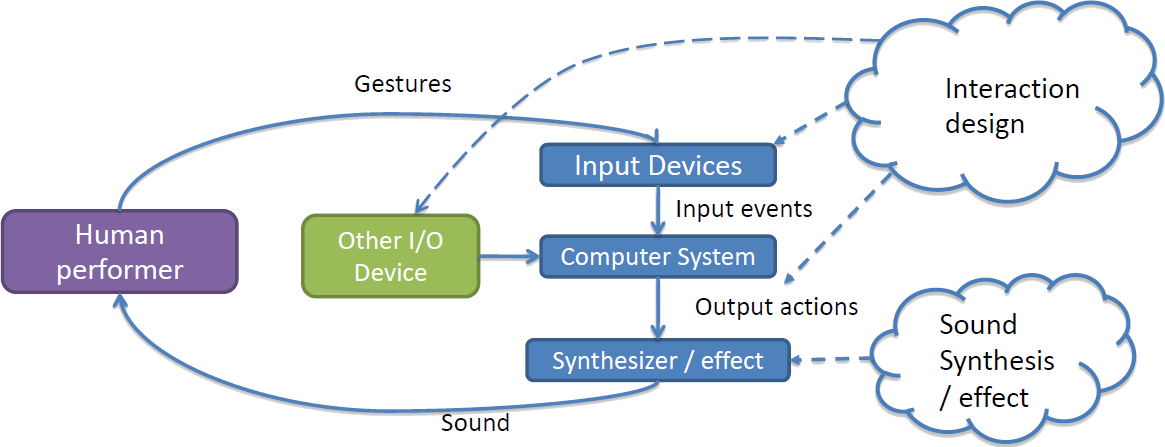
\includegraphics[width=0.8\linewidth]{00_Images/Res/05_chapter/01_cmps.png}
    \caption{Computer Music Performance System}
    \label{fig:computermusicperformancesystem}
\end{figure}

A Computer Music Performance System (CMPS) provides an interface between human performers and digitally controlled output devices. It consists of several key components:

\section{Components of a CMPS}

\begin{itemize}
    \item Human performer: Generates musical gestures while listening to the system’s output.
    \begin{itemize}
        \item Discrete gestures (e.g., pressing a key)
        \item Continuous gestures (e.g., varying pressure on a key)
    \end{itemize}
    \item Input device: Converts performance gestures into digital signals.
    \begin{itemize}
        \item Examples: computer keyboard, MIDI controller, motion sensors
    \end{itemize}
    \item Computer system: Processes input from devices and generates corresponding output actions.
    \begin{itemize}
        \item Can integrate additional input sources, such as external controllers
    \end{itemize}
    \item Synthesizer or effect processor: Receives commands from the computer system and generates or modifies audio waveforms.
\end{itemize}

\section{Applications of CMPS}

Computer Music Performance Systems enable various applications, including:

\begin{itemize}
    \item Virtual instruments
    \item Real-time composition
    \item Automated accompaniment
    \item Interactive performance environments
\end{itemize}

To support these applications, a CMPS must be programmable. The software environment of a CMPS typically includes:

\begin{itemize}
    \item One or more programming languages for defining musical interactions
    \item A real-time operating system that supports the semantic requirements of the language
\end{itemize}

\section{Real-Time Computer Music Systems}

A real-time system is one where system behavior depends on timing constraints. Real-time computer music systems must ensure low latency and precise timing for sound synthesis and interaction.

\section{Implementation of Computer Music Systems}

A computer music system consists of several interconnected components:

\paragraph{Hardware and Software Integration}

\begin{itemize}
    \item Personal Computer: The central processing unit for audio computation
    \item MIDI: Handles generation, recording, and playback of MIDI signals
    \item Audio: Manages sound synthesis, editing, recording, and playback
    \item Synthesizers: Can be implemented as:
    \begin{itemize}
        \item Software-based (internal)
        \item Hardware-based (external)
    \end{itemize}
\end{itemize}

\begin{figure}[!htb]
    \centering
    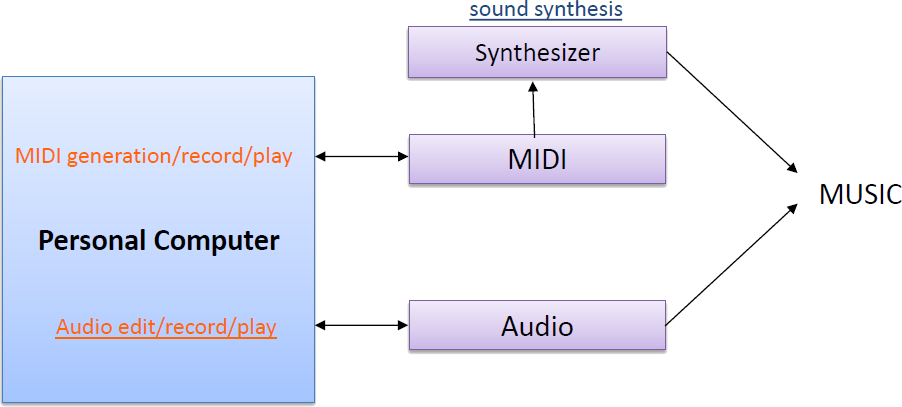
\includegraphics[width=0.8\linewidth]{00_Images/Res/05_chapter/02_cmsimplementation.png}
    \caption{Hardware and software integration}
    \label{fig:implementation01}
\end{figure}

\paragraph{System Architecture}

A computer music system includes multiple layers:

\begin{itemize}
    \item Software application: The user interface and main processing logic
    \item Kernel driver: Provides low-level access to audio hardware
    \item Sound card hardware: Processes and converts digital audio signals
    \item API and driver interaction: Manages communication between software and hardware
    \begin{itemize}
        \item Common APIs: PortAudio, PortMIDI, JACK, Core Audio
        \item Plugin standards: VST, Audio Unit
    \end{itemize}
\end{itemize}

\begin{figure}[!htb]
    \centering
    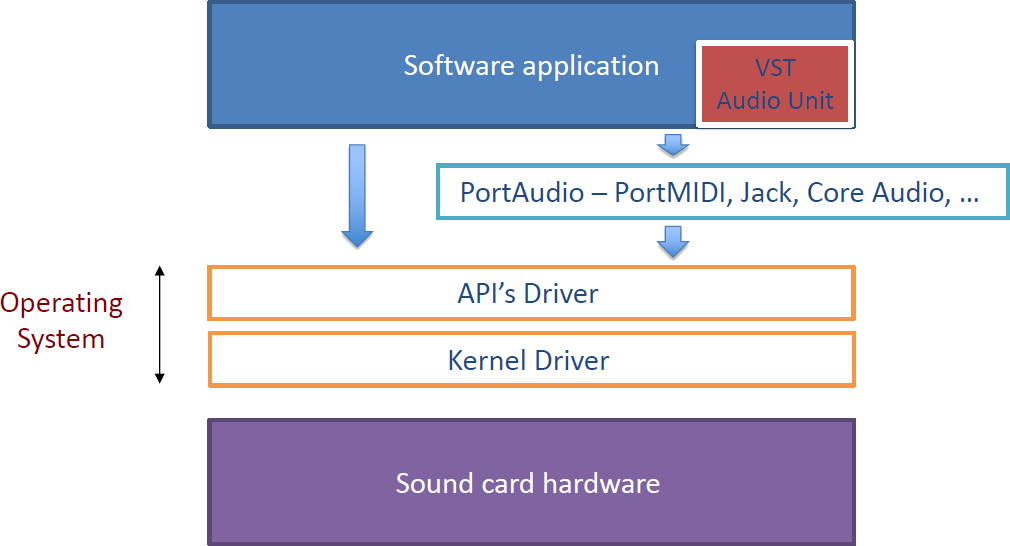
\includegraphics[width=0.8\linewidth]{00_Images/Res/05_chapter/03_cmsimplementation.png}
    \caption{System architecture}
    \label{fig:implementation02}
\end{figure}

\section{Sequencers and Their Role in Composition}

Sequencers play a fundamental role in the composition process by managing and organizing musical data. The composition process typically begins with MIDI (Musical Instrument Digital Interface) data, which consists of:

\begin{itemize}
    \item Notes
    \item Controller events
    \item Pitch bends
\end{itemize}

Modern sequencers allow for the recording of both MIDI data and digital audio from various sources, including:

\begin{itemize}
    \item MIDI devices (e.g., synthesizers, drum machines)
    \item Live instruments
    \item Vocal recordings
\end{itemize}

Once a musical project is stored as digital audio, it can be edited and processed with sound editing tools. Effects can be applied in real-time or offline to enhance the final output.

\subsection{Life-Cycle of a Composition in a Sequencer}

The composition process follows a structured flow:

\begin{enumerate}
    \item Musical data acquisition: Capturing notes, controller events, and pitch bends.
    \item Audio recording: Converting MIDI performances and live recordings into digital audio.
    \item Editing and processing: Modifying, arranging, and refining recorded material.
    \item Mixing and effects: Applying digital effects and balancing audio levels.
    \item Final rendering: Exporting the completed composition as a high-quality audio file.
\end{enumerate}

\begin{figure}[!htb]
    \centering
    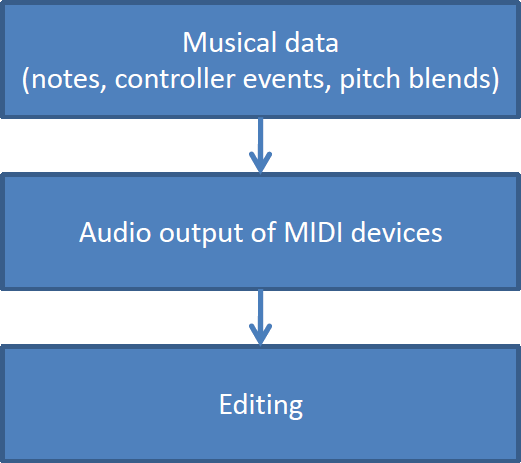
\includegraphics[width=0.7\linewidth]{00_Images/Res/05_chapter/04_sequencers.png}
    \caption{Life-cycle of a composition}
    \label{fig:life-cyclecomposition}
\end{figure}

\section{Signal Processing in Computer Music Systems}

Computer Music Performance Systems require efficient audio processing capabilities. Signal processing tasks can be divided into two categories:

\begin{itemize}
    \item Effect processing: Requires both input and output to modify an existing signal.
    \item Sound synthesis: Requires only an output to generate new sounds.
\end{itemize}

Signal processing systems integrate data acquisition hardware with microprocessors to execute algorithms on audio data. 

\begin{figure}[!htb]
    \centering
    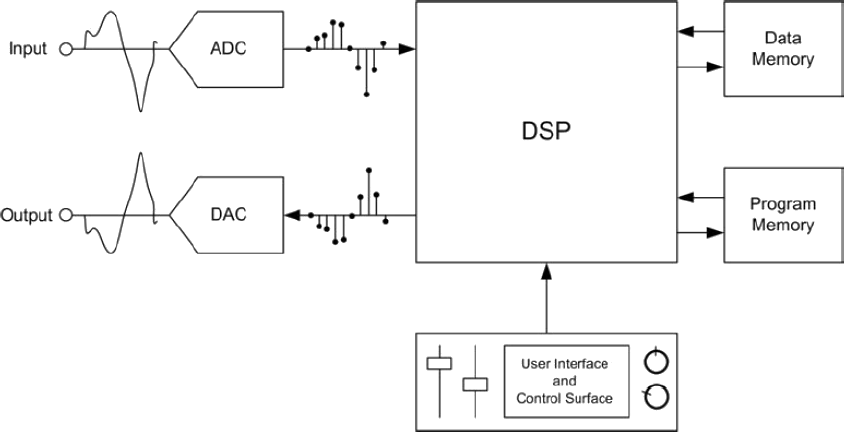
\includegraphics[width=0.8\linewidth]{00_Images/Res/05_chapter/05_signalprocessingsystem.png}
    \caption{Signal processing systems}
    \label{fig:signalprocessingsystems}
\end{figure}

\subsection{Effect Processor Architecture}

An effect processor typically consists of:

\begin{itemize}
    \item Digital Signal Processor (DSP): Specialized hardware optimized for real-time audio processing.
    \item User Interface (UI): Controls for modifying processing parameters, such as knobs and buttons.
    \item Program Memory: Stores the DSP program code.
    \item Data Memory: Stores input and processed audio data.
\end{itemize}

\subsection{DSP Execution Process}

DSPs operate efficiently by employing:

\begin{itemize}
    \item Multiply-and-accumulate operations as the core computational unit.
    \item Pipelining techniques to fetch new data while processing existing data.
\end{itemize}

\subsection{Music Synthesis Devices}

A music synthesis device is an embedded system that integrates a CPU and a DSP:

\begin{itemize}
    \item The microcontroller handles user input and controls.
    \item The DSP executes synthesis and effects algorithms.
\end{itemize}

\begin{figure}
    \centering
    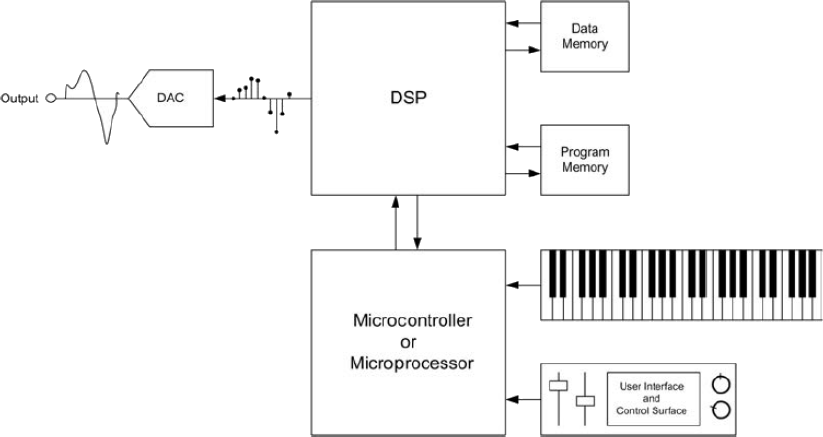
\includegraphics[width=0.8\linewidth]{00_Images/Res/05_chapter/06_signalprocessingsystem.png}
    \caption{Music synthesis system}
    \label{fig:musicsynthesissystem}
\end{figure}

\subsection{Signal Processing Flow}

The typical signal processing flow follows these steps:

\begin{enumerate}
    \item Initialization: Sets up the system and prepares for incoming data.
    \item Idle loop: Waits for an interrupt signal to process new data.
    \item Interrupt handling: Detects and decodes data interrupts.
    \item Data acquisition: Reads control and audio input data.
    \item Processing: Applies effects or synthesis algorithms to the audio signal.
    \item Output update: Adjusts parameters for the next processing cycle based on user input.
\end{enumerate}

Although traditionally performed on dedicated DSP hardware, this processing flow also applies to software-based implementations running on general-purpose computers.

\begin{figure}[!htb]
    \centering
    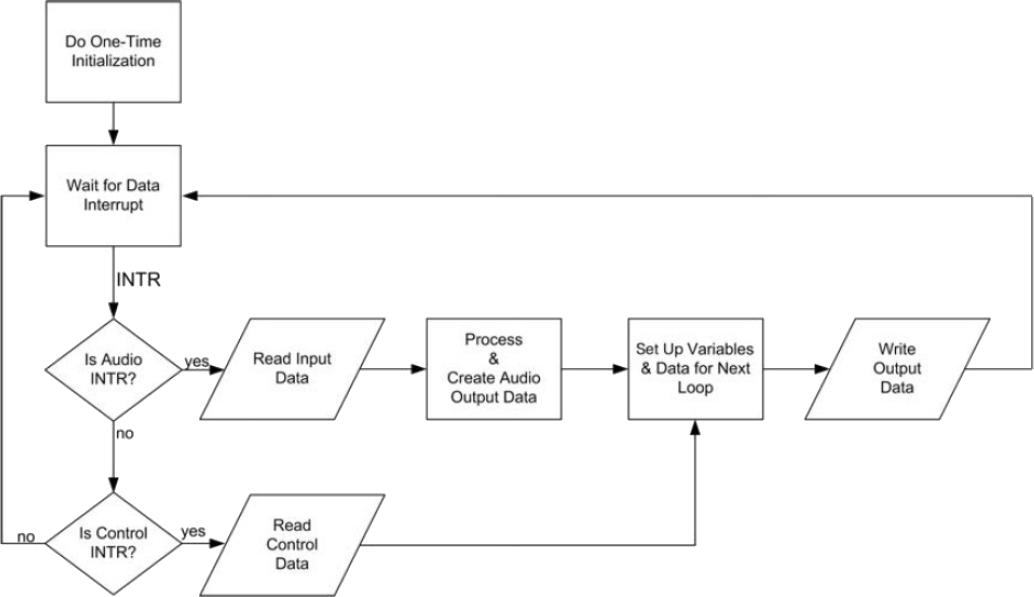
\includegraphics[width=0.8\linewidth]{00_Images/Res/05_chapter/07_signalprocessingflow.png}
    \caption{Signal processing flow}
    \label{fig:signalprocessingflow}
\end{figure}

\section{Plugins in Computer Music Systems}

A plugin is a software component that extends the functionality of another software application, referred to as the client. In computer audio systems, plugins serve various purposes, including:

\begin{itemize}
    \item Audio effects such as reverb, equalization, and distortion
    \item Signal analysis tools like oscilloscopes and spectrum analyzers
    \item Virtual instruments that function as synthesizers
\end{itemize}

\subsection{Interaction Between Plugins and the Client}

The communication method between a plugin and its client varies depending on the operating system:

\begin{itemize}
    \item Windows plugins are typically distributed as Dynamic Link Library (DLL) files.
    \item macOS plugins are packaged as bundles configured as components.
\end{itemize}

For simplicity, we refer to all dynamically linked plugins as DLLs.

\subsection{Static vs. Dynamic Linking}

\begin{itemize}
    \item Static linking: The plugin’s functions are compiled directly into the client application.
    \item Dynamic linking: The plugin exists as a separate file, and a communication mechanism is required to interact with the client.
\end{itemize}

Dynamic linking allows new functionalities to be added to a Digital Audio Workstation (DAW) without requiring recompilation.

\begin{figure}[!htb]
    \centering
    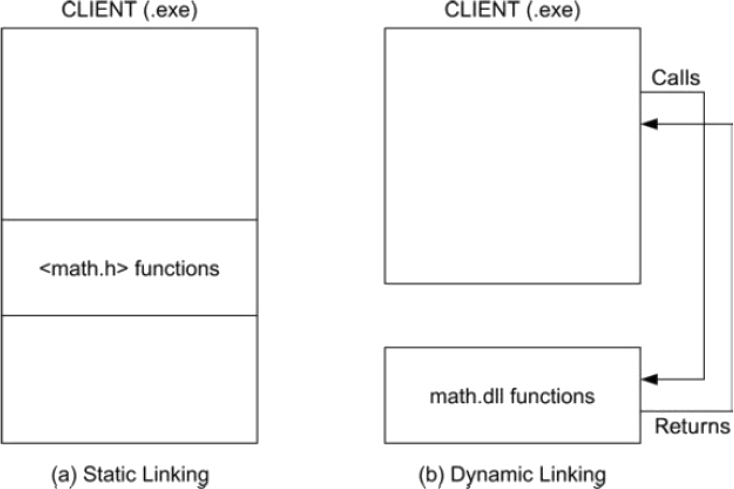
\includegraphics[width=0.6\linewidth]{00_Images/Res/05_chapter/08_plugins.png}
    \caption{Static vs. dynamic linking}
    \label{fig:staticdynamic}
\end{figure}

\subsection{Dynamic Link Library (DLL) Mechanism}

A DLL that shares the same process memory as the client requires the following steps to function:

\begin{enumerate}
    \item The client loads the DLL into its process address space.
    \item A communication mechanism is established between the client and the DLL functions.
    \item The client calls functions in the DLL as needed.
\end{enumerate}

In Windows, the following functions are used:

\begin{itemize}
    \item \texttt{LoadLibrary()}: Loads the DLL into memory.
    \item \texttt{GetProcAddress()}: Retrieves pointers to specific functions in the DLL.
    \item \texttt{FreeLibrary()}: Unloads the DLL when it is no longer needed.
\end{itemize}

\subsection{Implementation in C and C++}

\paragraph{C-style DLLs} In C, DLLs are implemented as collections of stand-alone functions without a \texttt{main()} function. To store persistent data:

\begin{itemize}
    \item A data structure is allocated using \texttt{malloc()} during initialization.
    \item A pointer to this structure is passed to the client for subsequent calls.
\end{itemize}

\begin{figure}[!htb]
    \centering
    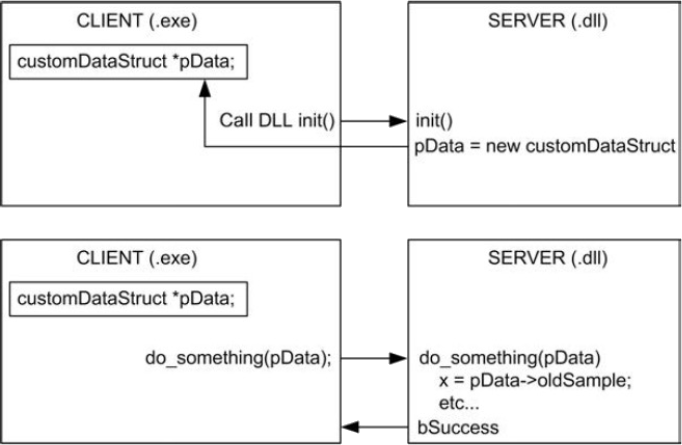
\includegraphics[width=0.6\linewidth]{00_Images/Res/05_chapter/09_plugins.png}
    \caption{C style DLL}
    \label{fig:cstyle}
\end{figure}

\paragraph{C++ style DLLs} In C++, DLLs take advantage of object-oriented programming:

\begin{itemize}
    \item Instead of allocating a data structure manually, the DLL creates an instance of a plugin object.
    \item The client interacts with the plugin by calling methods on this object.
    \item Multiple instances of the same plugin can be created and managed efficiently.
\end{itemize}

\begin{figure}[!htb]
    \centering
    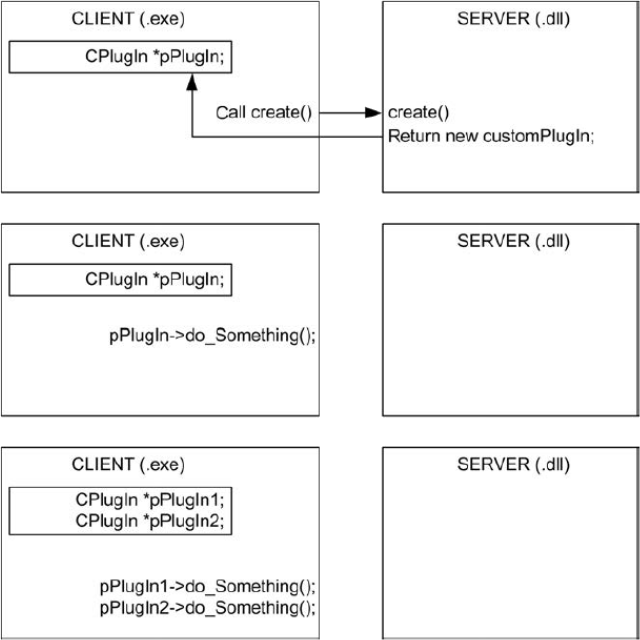
\includegraphics[width=0.6\linewidth]{00_Images/Res/05_chapter/10_plugins.png}
    \caption{C++ style DLL}
    \label{fig:c++style}
\end{figure}

\section{Graphical User Interface (GUI) for Plugins}

Most plugins include a GUI to control parameters. The GUI can be managed in three different ways:

\begin{enumerate}
    \item The client creates, maintains, and destroys the GUI, forwarding parameter changes to the plugin.
    \item The client creates and maintains the GUI, but the GUI directly communicates parameter changes to the plugin.
    \item The plugin itself handles the GUI and parameter communication.
\end{enumerate}

\subsection{GUI Management Strategies}

\paragraph{Client-Controlled GUI}

\begin{itemize}
    \item The client application is responsible for creating and managing the GUI.
    \item Control changes are forwarded to the plugin.
    \item This approach allows the client to have full control over GUI consistency.
\end{itemize}

\begin{figure}[!htb]
    \centering
    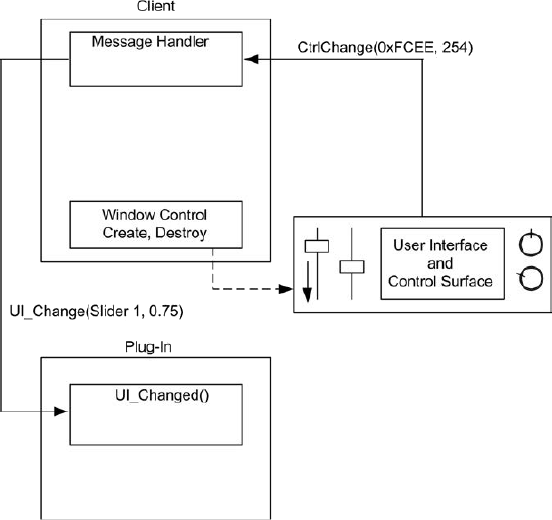
\includegraphics[width=0.6\linewidth]{00_Images/Res/05_chapter/11_userinterface.png}
    \caption{Client-controlled GUI}
    \label{fig:clientcontrolledgui}
\end{figure}

\paragraph{Client-Controlled GUI with Direct Plugin Communication}

\begin{itemize}
    \item The client creates the GUI but allows it to communicate directly with the plugin.
    \item This approach reduces the number of forwarded messages, improving efficiency.
\end{itemize}

\begin{figure}[!htb]
    \centering
    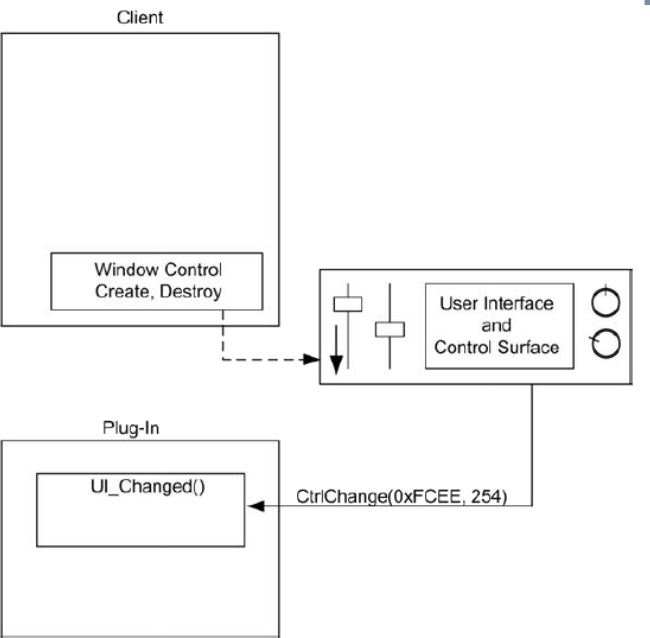
\includegraphics[width=0.6\linewidth]{00_Images/Res/05_chapter/12_userinterface.png}
    \caption{Client-controlled GUI with Direct Plugin Communication}
    \label{fig:clientcontrolledguiwithdirectplugincomm}
\end{figure}

\paragraph{Plugin-Controlled GUI}

\begin{itemize}
    \item The plugin creates and manages its own GUI.
    \item This provides more flexibility but requires the plugin to handle GUI updates and interactions.
\end{itemize}

\begin{figure}[!htb]
    \centering
    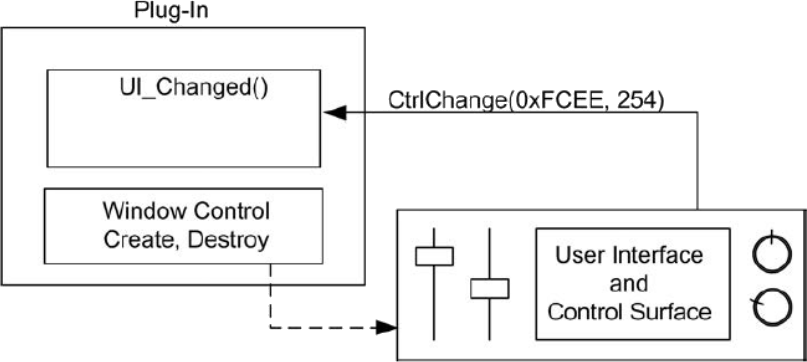
\includegraphics[width=0.6\linewidth]{00_Images/Res/05_chapter/13_userinterface.png}
    \caption{Plugin-controlled GUI}
    \label{fig:plugincontrolledgui}
\end{figure}

\section{Plugin Structure and API}

A plugin must implement a minimal set of functions defined by the Application Programming Interface (API) to interact with the client. The API ensures:

\begin{itemize}
    \item Compatibility across different versions of the client software.
    \item A standardized set of functions that all plugins must implement.
\end{itemize}

Object-oriented programming simplifies API integration:

\begin{itemize}
    \item If the plugin is an instance of an abstract base class defined by the client manufacturer, the API functions are guaranteed to be implemented.
\end{itemize}

\subsection{Core Plugin Operations}

Common functions shared across plugin APIs include:

\begin{itemize}
    \item Initialization and shutdown
    \item Audio processing
    \item Parameter management
    \item GUI handling
\end{itemize}  % Chapter 5
    %! TEX root = main.tex  % Specifies the main document file for multi-file projects

\chapter{Introduction to JUCE}

JUCE is a cross-platform C++ framework designed for audio applications and plugin development. Projucer is an integrated project management tool that simplifies JUCE-based development.

Key features of Projucer:

\begin{itemize}
    \item Supports multiple operating systems (Windows, macOS, Linux, iOS, Android)
    \item Generates project files compatible with popular IDEs (Xcode, Visual Studio, Makefile)
    \item Manages project settings, source files, and dependencies
    \item Provides a live build feature for real-time code compilation and preview
\end{itemize}

Projucer organizes projects using predefined templates, which can be further modified in an external IDE.

\section{Workflow of Application Development with JUCE}

The general workflow for developing an application with JUCE includes:

\begin{enumerate}
    \item Setting up the project using Projucer
    \item Including the required JUCE and external libraries
    \item Developing, building, and deploying the project in the preferred IDE
\end{enumerate}

When using the live build functionality, the build and development process can be completed within Projucer.

\section{Project Types in Projucer}

Projucer supports several types of projects, each suited for different applications:

\begin{itemize}
    \item GUI Application: A minimal JUCE project with an empty application window, used for graphical user interface development.
    \item Animated Application: Similar to a GUI application but optimized for graphical animations.
    \item OpenGL Application: Adds OpenGL support for rendering 3D graphics and shaders.
    \item Console Application: A command-line application without a graphical interface.
    \item Audio Application: A project pre-configured for audio input and output handling.
    \item Audio Plug-In: A template for VST, AudioUnit, and AAX plugin development.
    \item Static Library: Used to create reusable software libraries linked statically.
    \item Dynamic Library: Similar to a static library but linked dynamically.
\end{itemize}

\section{Example Projects in Projucer}

JUCE provides example projects located in the \texttt{JUCE/examples} directory. These projects serve as templates and can be accessed via:

\begin{supercollider*}
File > Open Example
\end{supercollider*}

\section{Audio Plugin Development with JUCE}

\subsection{Core Plugin Classes}

A JUCE audio plugin project is built around two main classes:

\begin{itemize}
    \item \texttt{nameOfTheProjectAudioProcessor}: Inherits from \texttt{AudioProcessor} and handles audio processing and MIDI input/output.
    \item \texttt{nameOfTheProjectAudioProcessorEditor}: Inherits from \texttt{AudioProcessorEditor} and manages the plugin’s graphical user interface.
\end{itemize}

These classes implement a communication mechanism between the Digital Audio Workstation (DAW) and the plugin.

\subsection{Key Methods in the AudioProcessor Class}

The \texttt{AudioProcessor} class defines the core functionality of the plugin:

\begin{itemize}
    \item \texttt{nameOfTheProjectAudioProcessor()}: Constructor
    \item \texttt{\textasciitilde nameOfTheProjectAudioProcessor()}: Destructor
    \item \texttt{void prepareToPlay(double sampleRate, int samplesPerBlock) override}: Initializes the processor
    \item \texttt{void processBlock(AudioBuffer<float>\&, MidiBuffer\&) override}: Handles audio and MIDI processing
    \item \texttt{void releaseResources() override}: Cleans up resources when the plugin is deactivated
\end{itemize}

\subsection{Key Methods in the AudioProcessorEditor Class}

The \texttt{AudioProcessorEditor} class is responsible for rendering the GUI:

\begin{itemize}
    \item \texttt{nameOfTheProjectAudioProcessorEditor(nameOfTheProjectAudioProcessor\&)}: Constructor
    \item \texttt{\textasciitilde nameOfTheProjectAudioProcessorEditor()}: Destructor
    \item \texttt{void paint(Graphics\&) override}: Renders visual elements
    \item \texttt{void resized() override}: Adjusts the layout when the window is resized
\end{itemize}

\section{Creating GUI Controls in the Plugin}

To add a new GUI control (e.g., a slider), the following steps must be followed:

\begin{enumerate}
    \item Declare the control as a private member in \texttt{AudioProcessorEditor}.
    \item Set the control properties.
    \item Use \texttt{addAndMakeVisible} to display the control in the plugin window.
    \item Adjust the control’s size and position in the \texttt{resized()} function.
    \item Attach a listener to update the controlled parameter when the control value changes.
\end{enumerate}

Example methods:

\begin{itemize}
    \item \texttt{AudioProcessorEditor::AudioProcessorEditor()}: Initializes the control
    \item \texttt{AudioProcessorEditor::resized()}: Adjusts control layout
    \item \texttt{AudioProcessorEditor::typeOfComponentValueChanged()}: Handles control interactions
\end{itemize}

Common GUI components include:

\begin{itemize}
    \item Button
    \item TextButton
    \item Slider (including rotary sliders)
    \item ComboBox
\end{itemize}
  % Chapter 6
    %! TEX root = main.tex  % Specifies the main document file for multi-file projects

\chapter{Analysis of a JUCE Project: SARAH Plugin}

The SARAH plugin (Synthèse à Rapide Analyse Harmonique) is an additive synthesizer that operates in the frequency domain. The official documentation and source code are available at:

\begin{itemize}
    \item \url{https://www.getdunne.net/wiki/doku.php?id=sarah}
    \item \url{https://github.com/getdunne/SARAH}
\end{itemize}

\begin{figure}[!htb]
    \centering
    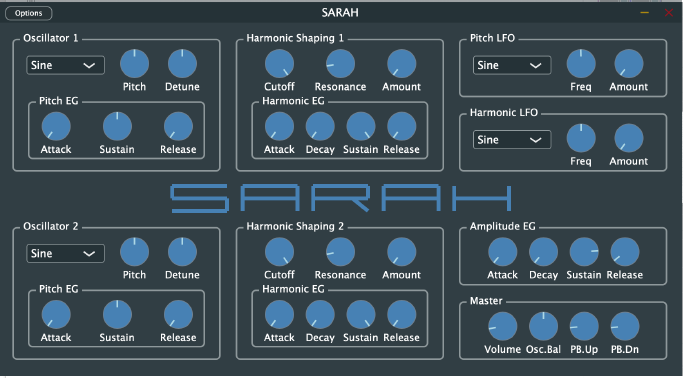
\includegraphics[width=0.8\linewidth]{00_Images/Res/07_chapter/01.png}
    \caption{SARAH plugin}
    \label{fig:sarah}
\end{figure}

\section{Main Features}

SARAH provides the following synthesis and modulation capabilities:

\begin{itemize}
    \item Two oscillators with selectable sinusoidal, square, sawtooth, and triangular waveshapes.
    \item Independent pitch and detuning controls for each oscillator.
    \item Harmonic shaping via frequency-domain filtering.
    \item ADSR amplitude envelope.
    \item ASR pitch envelope.
    \item Low-frequency oscillators (LFOs) for pitch and harmonic modulation.
    \item Global amplitude envelope.
\end{itemize}

\section{Functional Blocks in SARAH}

The plugin can be broken down into three primary functional blocks:

\begin{itemize}
    \item Oscillators: OSC1 and OSC2 generate fundamental audio signals and are instances of the \texttt{SynthOscillator} class.
    \item Low-Frequency Oscillators (LFOs): Used for pitch and harmonic modulation, implemented in the \texttt{SynthLFO} class.
    \item Envelope Generators: ShapeEG1, ShapeEG2, PitchEG1, PitchEG2, and AmpEG, all instances of \texttt{SynthEnvelopeGenerator}.
\end{itemize}

Both \texttt{SynthOscillator} and \texttt{SynthLFO} inherit from the base class \texttt{SynthBaseOscillator}, ensuring a common interface for signal generation.

\begin{figure}[!htb]
    \centering
    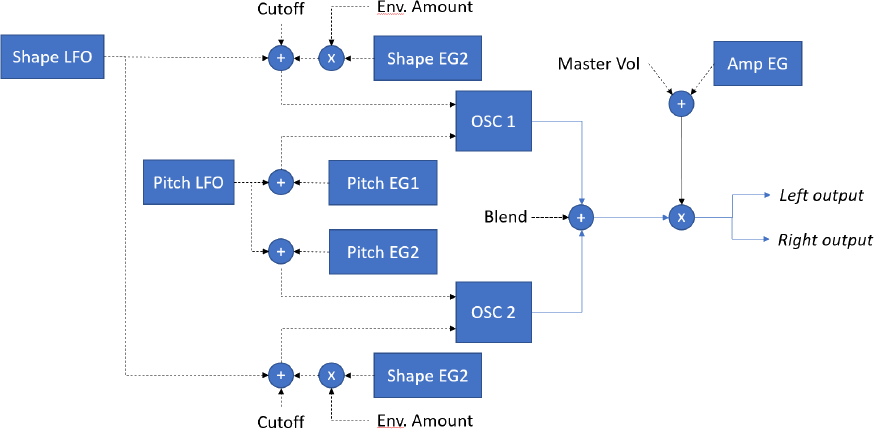
\includegraphics[width=0.7\linewidth]{00_Images/Res/07_chapter/02.png}
    \caption{Functional block}
    \label{fig:functionalblock}
\end{figure}

\section{Wavetable-Based Signal Generation}

\subsection{Wavetable Approach}

The plugin utilizes a wavetable approach for waveform generation. The fundamental concept is:

\begin{itemize}
    \item The square, sawtooth, and triangular waveforms are precomputed and stored in a wavetable.
    \item A fast Fourier transform (FFT) is applied to the waveform to generate its frequency-domain representation.
    \item A harmonic filter is applied, followed by an inverse FFT to reconstruct the waveform.
\end{itemize}

\begin{figure}[!htb]
    \centering
    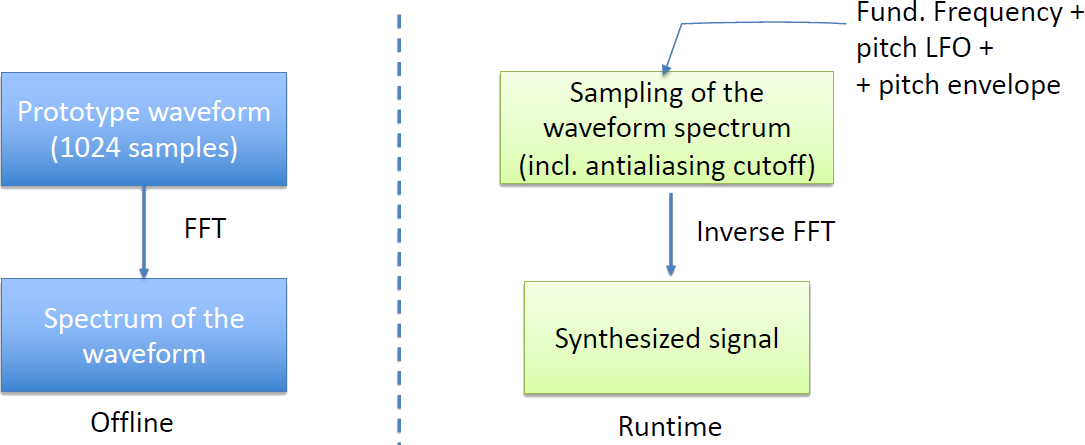
\includegraphics[width=0.6\linewidth]{00_Images/Res/07_chapter/03.png}
    \caption{Wavetable approach}
    \label{fig:wavetableapproach}
\end{figure}

\subsection{Wavetable Formulae}

The synthesized waveforms are generated using the following equations:

\begin{itemize}
    \item Triangle Wave:
    \[
    s(i) = 4 \times (0.5 - | \varphi - 0.5 |) - 1, \quad N = 1024
    \]
    \item Square Wave:
    \[
    s(i) =
    \begin{cases} 
      1 & \text{if } \varphi \leq 0.5 \\
      -1 & \text{if } \varphi > 0.5
    \end{cases}
    \]
    \item Sawtooth Wave:
    \[
    s(i) = 2\varphi - 1
    \]
\end{itemize}

\begin{figure}[!htb]
    \centering
    \subfloat{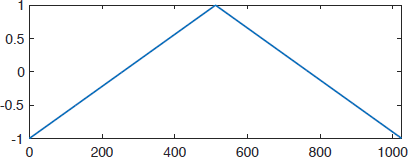
\includegraphics[width=0.3\linewidth]{00_Images/Res/07_chapter/04.png}}\hfill
    \subfloat{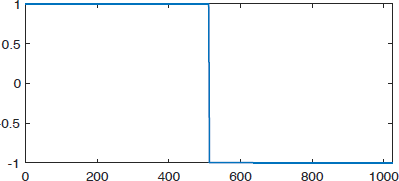
\includegraphics[width=0.3\linewidth]{00_Images/Res/07_chapter/05.png}}\hfill
    \subfloat{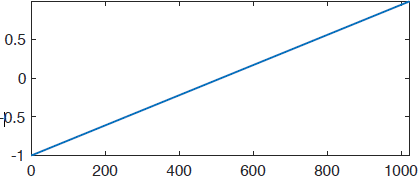
\includegraphics[width=0.3\linewidth]{00_Images/Res/07_chapter/06.png}}
    \caption{Wavetable formulae graphs}
    \label{fig:wavetableformulaegraphs}
\end{figure}

\subsection{Implementation in SARAH}

To generate a waveform at the correct frequency, SARAH follows this approach:

\begin{itemize}
    \item Instead of performing time-domain interpolation, the spectrum of the prototype waveform is sampled and zero-padded.
    \item The actual waveform is generated every time:
    \begin{itemize}
        \item A new note is played.
        \item Pitch is modulated by the LFO.
        \item The plugin starts.
    \end{itemize}
\end{itemize}

\section{Low-Frequency Oscillator (LFO)}

LFOs are used to modulate pitch and harmonic content. The \texttt{SynthLFO} class inherits from \texttt{SynthOscillatorBase} and generates:

\begin{itemize}
    \item Sine waves
    \item Square waves
    \item Triangle waves
    \item Sawtooth waves
\end{itemize}

Unlike audio oscillators, LFOs use a phase-offset technique instead of wavetable interpolation.

\section{Envelope Generator}

\subsection{Purpose of the Envelope Generator}

The \texttt{SynthEnvelopeGenerator} class modulates:

\begin{itemize}
    \item Pitch
    \item Formant filter parameters
    \item Amplitude of the synthesized waveform
\end{itemize}

\subsection{Envelope States}

The envelope has four states:

\begin{itemize}
    \item Idle
    \item Attack
    \item Decay
    \item Sustain
    \item Release
\end{itemize}

SARAH uses the JUCE \texttt{LinearSmoothedValue} class for linear interpolation between values.

\section{Managing Polyphony}

SARAH supports 16 simultaneous voices across 128 program banks. Polyphony is handled using three JUCE classes:

\begin{itemize}
    \item \texttt{Synthesiser}: Manages voices and sound programs.
    \item \texttt{SynthesiserVoice}: Represents a single voice, containing oscillators and envelope generators.
    \item \texttt{SynthesiserSound}: Defines the sound properties assigned to a synthesizer.
\end{itemize}

\subsection{Voice Allocation}

Each new note is assigned to an available voice. The plugin uses an internal voice-stealing mechanism to reallocate voices when necessary.

\section{Audio Processor Integration}

The \texttt{SARAHAudioProcessor} class integrates the synthesizer within the plugin framework. Key functions include:

\begin{itemize}
    \item \texttt{processBlock()}: Processes incoming MIDI messages and generates audio output.
    \item \texttt{getSound()}: Retrieves the current sound settings.
\end{itemize}

\section{Customizing the GUI}

\subsection{JUCE LookAndFeel}

The GUI appearance can be customized using the JUCE \texttt{LookAndFeel} class. This allows:

\begin{itemize}
    \item Customizing colors of UI components.
    \item Redefining how sliders, buttons, and other elements are drawn.
\end{itemize}

\subsection{Example: Custom Rotary Slider}

A rotary slider can be customized by overriding the \texttt{drawRotarySlider} function:

\begin{supercollider*}
void drawRotarySlider (juce::Graphics& g, int x, int y, int width, 
int height, float sliderPos, const float rotaryStartAngle, 
const float rotaryEndAngle, juce::Slider&) override
{
    auto radius = (float) juce::jmin (width / 2, height / 2) - 4.0f;
    auto centreX = (float) x + (float) width  * 0.5f;
    auto centreY = (float) y + (float) height * 0.5f;
    auto angle = rotaryStartAngle + sliderPos * (rotaryEndAngle - rotaryStartAngle);

    g.setColour (juce::Colours::orange);
    g.fillEllipse (centreX - radius, centreY - radius, radius * 2, radius * 2);
}
\end{supercollider*}

\section{Conclusions}

When developing or analyzing a JUCE plugin, it is essential to:

\begin{itemize}
    \item Clearly define the plugin’s purpose and behavior.
    \item Use existing DSP implementations to validate concepts before coding in C++.
    \item Recognize standard plugin architectures to simplify reverse engineering.
\end{itemize}
  % Chapter 7
    


\end{document}